% ch05-frame-by-frame.tex — Frame-by-frame forward chaining on the Mechanism KG.
% Shows G0 -> G1 -> G2 -> G3=G2 (fixpoint) with the three Datalog rules r1,r2,r3.
% Grayscale-safe: new triples carry BOTH a color AND a "+moi" text tag.
\documentclass[tikz,border=6pt]{standalone}
\usepackage{fontspec}
\setmainfont{Times New Roman}
\usepackage{unicode-math}
\setmathfont{Cambria Math}
\usetikzlibrary{positioning,arrows.meta}

\begin{document}
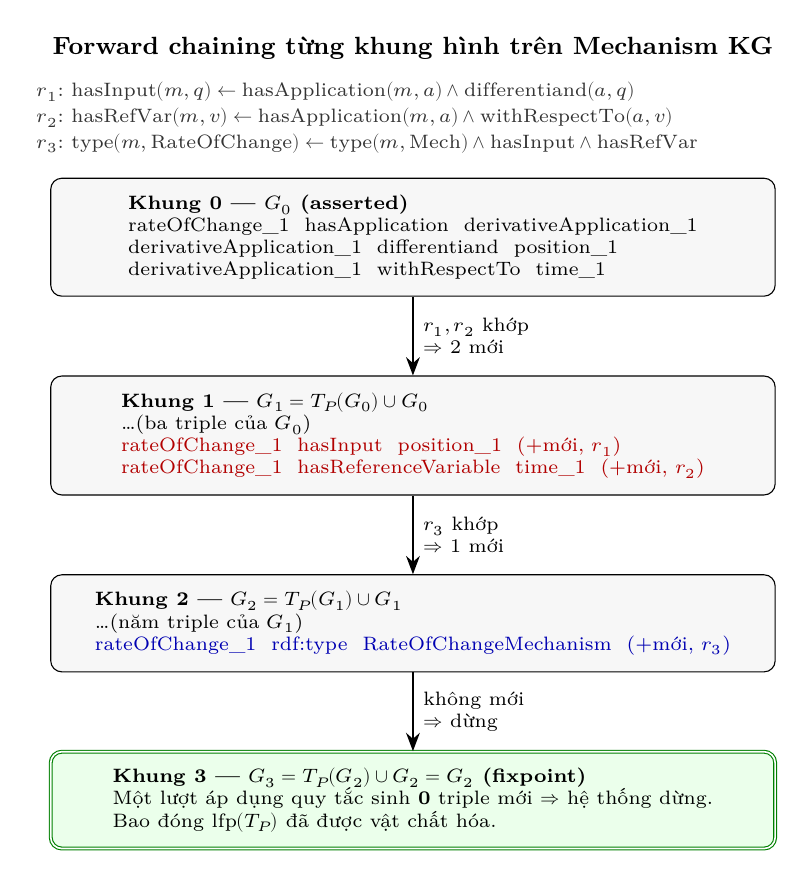
\begin{tikzpicture}[
  frame/.style={draw,rounded corners,inner sep=6pt,minimum width=9.2cm,align=left,
                font=\scriptsize},
  title/.style={font=\small\bfseries},
  arr/.style={->,>=Stealth,thick},
  rule/.style={font=\scriptsize,text=gray!40!black},
]

% Title + rules legend
\node[title] at (0,3.7) {Forward chaining từng khung hình trên Mechanism KG};
\node[rule,anchor=west] at (-4.9,3.15)
  {$r_1$:\ $\mathrm{hasInput}(m,q)\leftarrow \mathrm{hasApplication}(m,a)\wedge \mathrm{differentiand}(a,q)$};
\node[rule,anchor=west] at (-4.9,2.82)
  {$r_2$:\ $\mathrm{hasRefVar}(m,v)\leftarrow \mathrm{hasApplication}(m,a)\wedge \mathrm{withRespectTo}(a,v)$};
\node[rule,anchor=west] at (-4.9,2.49)
  {$r_3$:\ $\mathrm{type}(m,\mathrm{RateOfChange})\leftarrow \mathrm{type}(m,\mathrm{Mech})\wedge \mathrm{hasInput}\wedge \mathrm{hasRefVar}$};

% Frame 0
\node[frame,fill=gray!6] (F0) at (0,1.3) {%
  \textbf{Khung 0 --- $G_0$ (asserted)}\\
  rateOfChange\_1\ \ hasApplication\ \ derivativeApplication\_1\\
  derivativeApplication\_1\ \ differentiand\ \ position\_1\\
  derivativeApplication\_1\ \ withRespectTo\ \ time\_1};

% Frame 1
\node[frame,fill=gray!6,below=1.0cm of F0] (F1) {%
  \textbf{Khung 1 --- $G_1 = T_P(G_0)\cup G_0$}\\
  \dots (ba triple của $G_0$)\\
  \textcolor{red!70!black}{rateOfChange\_1\ \ hasInput\ \ position\_1\ \ (+mới, $r_1$)}\\
  \textcolor{red!70!black}{rateOfChange\_1\ \ hasReferenceVariable\ \ time\_1\ \ (+mới, $r_2$)}};

% Frame 2
\node[frame,fill=gray!6,below=1.0cm of F1] (F2) {%
  \textbf{Khung 2 --- $G_2 = T_P(G_1)\cup G_1$}\\
  \dots (năm triple của $G_1$)\\
  \textcolor{blue!70!black}{rateOfChange\_1\ \ rdf:type\ \ RateOfChangeMechanism\ \ (+mới, $r_3$)}};

% Frame 3
\node[frame,fill=green!8,draw=green!50!black,double,below=1.0cm of F2] (F3) {%
  \textbf{Khung 3 --- $G_3 = T_P(G_2)\cup G_2 = G_2$ (fixpoint)}\\
  Một lượt áp dụng quy tắc sinh \textbf{0} triple mới $\Rightarrow$ hệ thống dừng.\\
  Bao đóng $\mathrm{lfp}(T_P)$ đã được vật chất hóa.};

% Arrows
\draw[arr] (F0) -- node[right,font=\scriptsize,align=left] {$r_1,r_2$ khớp\\ $\Rightarrow$ 2 mới} (F1);
\draw[arr] (F1) -- node[right,font=\scriptsize,align=left] {$r_3$ khớp\\ $\Rightarrow$ 1 mới} (F2);
\draw[arr] (F2) -- node[right,font=\scriptsize,align=left] {không mới\\ $\Rightarrow$ dừng} (F3);

\end{tikzpicture}
\end{document}
